\section{Direct dense methods} \label{subseq:direct methods}
Direct methods have very good numerical stability properties. They do not require to modify a system of equations as it is necessary for iterative methods. Sometimes we only need to permute some rows and columns in order to avoid small absolute values along the matrix diagonal, which can have their negative effect on numerical accuracy, in case of direct methods. However, this operation can be considered relatively cheap. \\

On another hand, the computational complexity of $O(n^3)$ and storage requirements of $O(n^2)$ make direct methods not suitable for computation of large systems with more than $\sim 10^3$ number of equations. \\


Another good property of direct dense solvers is they have direct memory access and they are based on dense linear algebra subroutines. As a result, implementation of these methods can exploit such programming techniques like cache blocking, tiling, data prefetching,  utilization of hardware vector units and so on. All of these together make it possible to achieve more than 75\% hardware performance of modern CPUs \cite{articles:blas-performance} due to a high ratio of floating point operations per memory access. \\

A general way to solve a system of a type \ref{eq:slq} is to perform $LU$ factorization where a matrix $A$ can be viewed as a product of a lower and upper triangular matrices. 

\begin{equation} \label{eq:lu}
	Ax = LUx = b
\end{equation}

Having computed matrices $L$ and $U$, two additional steps, forward and backward substitutions, are required to compute the solution vector $x$.

\begin{align} \label{eq:bk}
	Ly = b \\
	Ux = y
\end{align}

The main idea of parallel $LU$ decomposition is based on block structure of a matrix $A$. Any given matrix $A$ can be represented as a combination of sub-matrices $A_{ij}$.

$$
A = 
\Bigg(\begin{array}{c|c|c}
A_{11} & A_{12} & A_{13} \\ \hline
A_{21} & A_{22} & A_{23} \\ \hline
A_{31} & A_{32} & A_{33}
\end{array}\Bigg)
$$

This allows to develop algorithms that can compute $LU$ decomposition of the full matrix $A$ in parallel using sub-matrices with three main routines i.e. matrix-matrix multiply, triangular solve with multiple right hand sides and the unblock $LU$ factorization for operation within a block column \cite{netlib:lapack-1}.\\

There exist three well known parallel approaches based on left, right and Crout decomposition forms. All of these three approaches have similar overall performance, with a slight advantage to the right-looking and Crout variants \cite{netlib:lapack-1}. 

% example

Let's consider right-looking algorithm as an example. The algorithm can be written as following:

\begin{equation} \label{eq:RightLookingLu}
\Bigg(\begin{array}{c c}
A_{11} & A_{12} \\
A_{21} & A_{22} \\
\end{array}\Bigg)
=
\Bigg(\begin{array}{c c}
L_{11} & 0 \\
L_{21} & L_{22} \\
\end{array}\Bigg)
\cdot
\Bigg(\begin{array}{c c}
U_{11} & U_{12} \\
0 & U_{22} \\
\end{array}\Bigg)
\end{equation}

The algorithm starts with an assumption that both matrices $L_{11}$ and $U_{11}$ have already been computed. 
% size of the matrix is proportional to the size of the cache

Given equation \ref{eq:RightLookingLu}, we can write expressions for $A_{12}$ and $A_{21}$ matrices:

\begin{align} \label{eq:RightLookingLuFirstUpdate}
A_{12} = L_{11} \cdot U_{12} \\
A_{21} = L_{21} \cdot U_{11}
\end{align}

To compute \ref{eq:RightLookingLuFirstUpdate} we only have to perform two triangular solves since matrices $L_{11}$ and $U_{11}$ are known. These two tasks are concurrent and they can be computed in parallel. Additionally we can notice the triangular solve routine can be computed in parallel too. The next step is to perform $\hat{A_{22}}$ matrix update and block structure re-odering:

\begin{equation} \label{eq:RightLookingLuSecondUpdate}
\hat{A_{22}} = A_{22} - L_{21} \cdot U_{12}
\end{equation}

\figpointer{\ref{fig:RightLookingLuReodering}}
\begin{figure}[htpb]
  \centering
  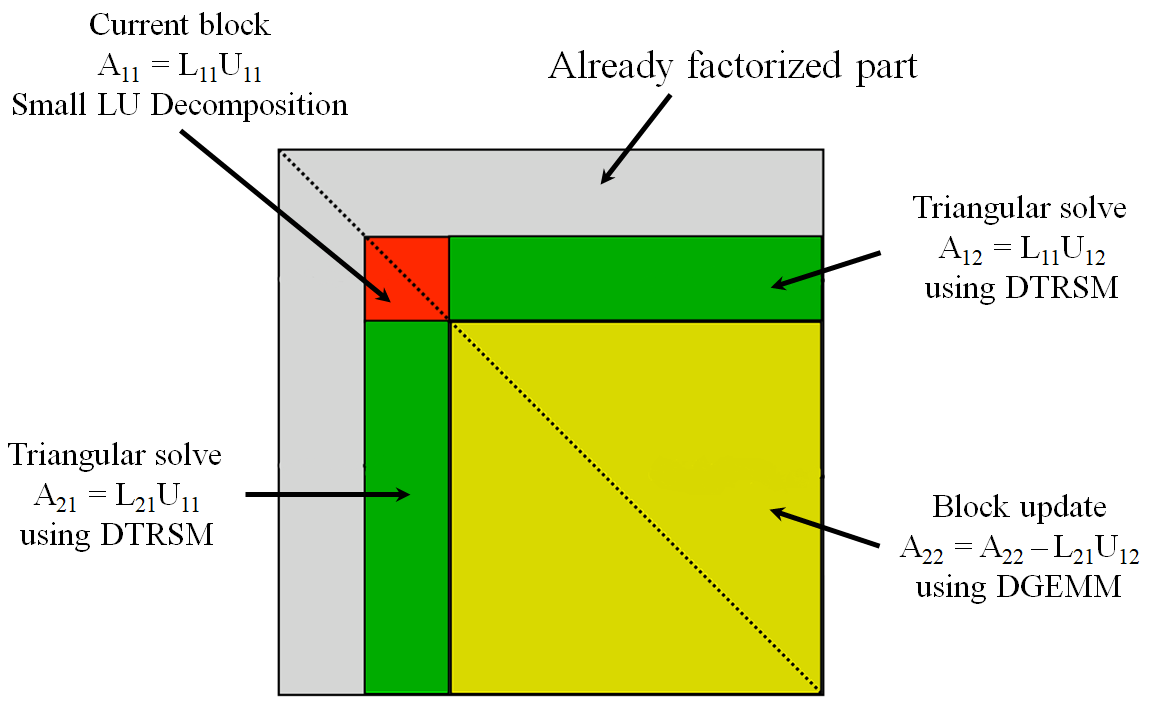
\includegraphics[width=0.75\textwidth]{figures/chapter-2/right-looking-la.png}
\caption{Right-looking parallel LU decomposition}
\label{fig:RightLookingLuReodering}
\end{figure}


% Show limited parallelism
It is clear the algorithm is purely sequential at the first steps when we compute small $LU$ decomposition. Therefore, it can have significant effect on algorithm strong scaling behavior. It should be mentioned that all three parallel implementations have the same problem i.e. they have an inherently sequential part at the beginning of a step. \\

Figure \ref{fig:lapack-lu-strong-scaling} shows results of strong scaling of dense $LU$ factorization performed for a couple of matrices filled with random numbers with different sizes: namely: $5000 \times 5000$, $10000 \times 10000$ and $15000 \times 15000$. LAPACK and OpenBLAS libraries were used for the test. One can easily notice that performance of dense $LU$ decomposition quickly deteriorates with reduction of the problem size. Additional factor that affects performance is strong scaling behavior of the triangular solve that we will discuss in section \ref{subseq:iterative methods}. 

\figpointer{\ref{fig:lapack-lu-strong-scaling}}
\begin{figure}[htpb]
  \centering
  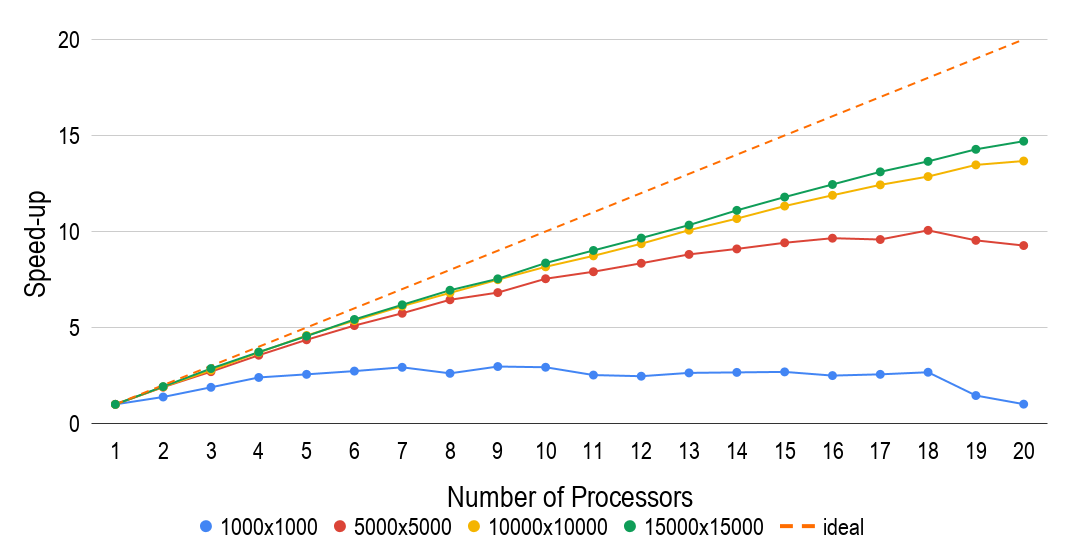
\includegraphics[width=0.85\textwidth]{figures/chapter-2/lapack-lu-strong-scaling.png}
\caption{Strong scaling of right-looking $LU$ decomposition using LAPACK and OpenBLAS}
\label{fig:lapack-lu-strong-scaling}
\end{figure}

% results of strong scaling

Both left, right and Crout parallel matrix factorizations have been efficiently implemented in LAPACK (for shared-memory machines) and ScaLAPACK (distributed-memory machines) libraries. Both libraries belong to the Netlib project which is a repository of numerous scientific computing software maintained by AT\&T Bell Laboratories, the University of Tennessee, Oak Ridge National Laboratory and other scintific communities \cite{netlib-overview}. The libraries are built on top of Basic Linear Algebra Subprograms (BLAS) library. Figure \ref{fig:blas-lapack-scalapack} shows how these three libraries are coupled together.\\


\figpointer{\ref{fig:blas-lapack-scalapack}}
\begin{figure}[htpb]
  \centering
  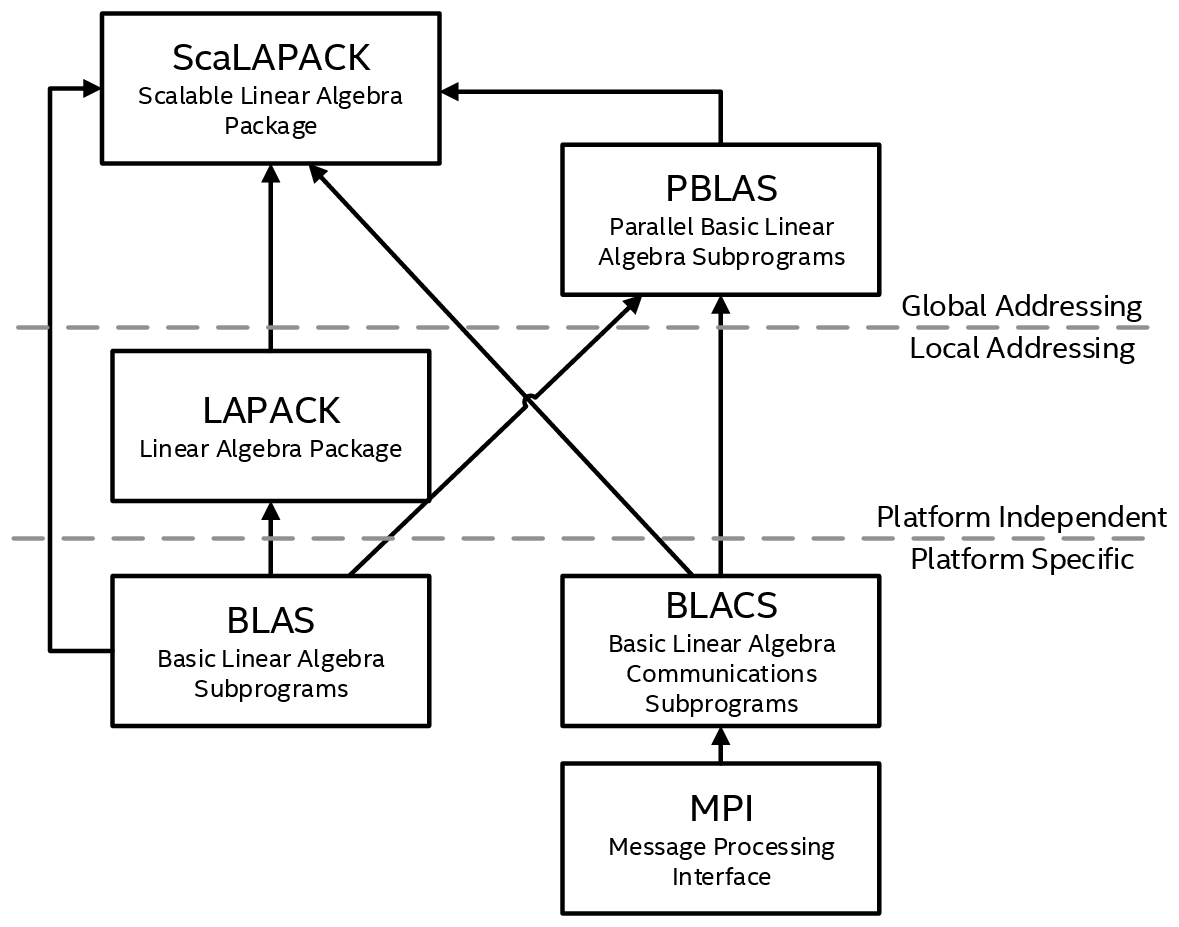
\includegraphics[width=0.65\textwidth]{figures/chapter-2/lapack-scalapack-blas.png}
\caption{A general view on BLAS, LAPACK and ScaLAPACK libraries \cite{netlib:lapack-scalapack-general-view}}
\label{fig:blas-lapack-scalapack}
\end{figure}

It is worth noting that BLAS can be considered as a foundation of LAPACK and ScaLAPACK libraries and, thus, it is the primary source of performance improvement. In particular we have to consider DGEMM, DTRSM BLAS subroutines performance because they, together with unblocked $LU$ factorization, compose the core of parallel $LU$ factorization algorithms as we discussed earlier.\\

There exist special-purpose, hardware-specific BLAS implementations developed by the hardware vendors i.e. IBM, Cray, Intel, AMD as well as open-source tuned implementations such as ATLAS, OpenBLAS, etc. We will come back to that discussion later and pay our close attention to a specific choice of a tuned BLAS library in subsection \ref{subseq:blas-comparison}.\\

In spite of all advantages of the direct dense solvers i.e. numerical stability and high ratio of floating point operations per memory access, we cannot consider this group of methods as a solver for time integration due to high complexity and storage costs.
